\begin{savequote}[45mm]
When I was in high school, my physics teacher called me down one day after
class and said, "You look bored, I want to tell you something interesting".
Then he told me something I have always found fascinating. Every time
the subject comes up I work on it.  
\qauthor{Richard Feynman}
\end{savequote}
\chapter{Analytical Mechanics}
\label{ch:method}
\section{Lagrangian Mechanics}
\begin{tcolorbox}
In the formulation of Lagrangian mechanics, we have the action functional
\begin{equation}
    S = \int^{b}_{a} L(x^{\mu}, {{x}^{'}}^{\mu}, t) \ dt
\end{equation}
the equations of motion are obtained when we stationarize the the action i.e. when we equate the Frechet derivative of the Lagrangian to . This produces $n$ $2^{\text{nd}}$ order non-linear (in most cases) partial differential equations. And generally for non-dissipative systems
\begin{equation}
    L = T - V
\end{equation}
Where $T$ is the kinetic energy of the system and $V$ the potential energy
\end{tcolorbox}
The advantages of using the Lagrangian mechanics are:
\begin{itemize}
    \item Scalars are used instead of vectors which makes calculations much easier
    \item The concept of forces is discarded and thus only knowledge of the kinetic and potential energy is required 
    \item Generalized coordinates are used thus, it is easier to transform to any arbitrary coordinate system (composed of only independent coordinates)
    \item Lagrangian mechanics holds for all frames of references, not just inertial frames
\end{itemize}
One key point however is that when we are talking about Lagrangian mechanics, we are not exactly talking about but rather a representation of it as the space of the arguments of the lagrangian for a system with $n$ independent coordinates lives in a $3n$ dimensional space called the configuration space
\begin{figure}[H]
    \centering
    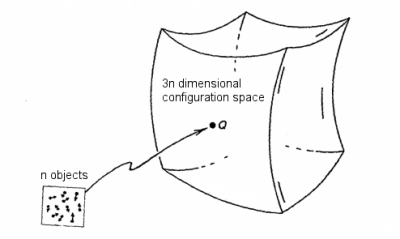
\includegraphics[scale=0.5]{Figures/configspace.png}
    \caption{A visualization of configuration space}
    \label{fig:my_label}
\end{figure}
\subsection{Constraints}
Holonomic constraints are relationships between the coordinates of the form
    \begin{align}
        f_{\alpha}(x^{\mu},t) = 0 \ \ , \ \ \alpha = 1,..,3N-n
    \end{align}
Holonomic constraints can be solved in terms of $n$ generalized coordinates $q_{i}$ where $i$ runs from $1$ to $n$. So 
\begin{equation}
    x^{\mu} = x^{\mu}(q_{1},..,q_{n})
\end{equation}
The system is said to have $n$ degrees of freedom. Let's take a look at an example
\begin{figure}[H]
    \centering
    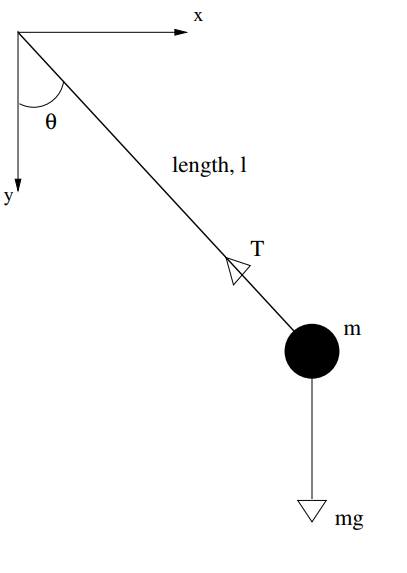
\includegraphics[scale=0.5]{Figures/pendulum.png}
    \caption{A Simple Pendulum}
    \label{fig:my_label}
\end{figure}
here the pendulum has a single degree of freedom, $q = \theta$. We have the equations of motion
    \begin{align}
        m\ddot{x} = -Tx/l \ \ , \ \ m \ddot{y} = mg - Ty/l
    \end{align}
and constraints
    \begin{align}
        \ddot{\theta} = -(g/l)sin(\theta) \ \ , \ \  T = ml\dot{\theta}^{2} + mg cos(\theta)
    \end{align}
Now let's see how we can solve this using the Lagrangian formalism. We start by introducing $3N-n$ new variables $\lambda_{\alpha}$, called Lagrange multipliers and define a new Lagrangian
\begin{equation}
    L^{'} = L(x^{\mu},\dot{x}^{\mu}) + \lambda_{\alpha} f_{\alpha}(x^{\mu},t)
\end{equation}
We treat $\lambda_{\alpha}$ like new coordinates. Since $L^{'}$ doesn't depend on $\dot{\lambda}_{\alpha}$, thus the Euler-Lagrange equations for $\lambda_{\alpha}$:
\begin{equation}
    \frac{\partial L^{'}}{\partial \lambda_{\alpha}} = f_{\alpha}(x^{\mu},t) = 0
\end{equation}
and the equations for the $x^{\mu}$ are
\begin{equation}
    \frac{d}{dt}\left( \frac{\partial L}{\partial \dot{x}^{\mu}} \right) - \frac{\partial L}{\partial x^{\mu}} = \lambda_{\alpha} \frac{\partial f_{\alpha}}{\partial x^{\mu}}
\end{equation}
Here the RHS represents the constrained system's equation of motion and the LHS the unconstrained one.
Let's have one more go at this problem, the Lagrangian for the pendulum is given by a free particle moving in a plane i.e. a circle
\begin{equation}
    L^{'} = \frac{1}{2}m(\dot{x}^{2} + \dot{y}^{2}) + mgy + \frac{1}{2}\lambda(x^{2} + y^{2} - l^{2})
\end{equation}
from which we get the equations of motion for $x$ and $y$,
\begin{equation}
    m \ddot{x} = \lambda x
\end{equation}
\begin{tcolorbox}
    \textbf{Theorem:} For constrained systems we may derive the equations directly in terms of the generalized coordinates $q_{i}$
    \begin{equation}
        L(q^{i},\dot{q}^{i}, t) = L(x^{\mu}(q^{i},t),\dot{x}^{\mu}(\dot{q}^{i}, t))
    \end{equation}
    \textbf{Proof:} Let's work with $L^{'} = L + \lambda_{\alpha}f_{\alpha}$ and change coordinates to:
    \begin{equation}
    x^{\mu} \rightarrow 
        \begin{cases}
            q_{i} \ \ \ & i = 1,...,n\\
f_{\alpha},            \ \ \  & \alpha = 1,...,3N-n
        \end{cases}
    \end{equation}
    We know that Lagrange's equations take the same form in these new coordinates
    \begin{equation}
        \frac{d}{dt}\left( \frac{\partial L}{\partial \dot{q}^{i}} \right) - \frac{\partial L}{\partial q^{i}} = \lambda_{\alpha} \frac{\partial f_{\alpha}}{\partial q^{i}}
    \end{equation}
    But, by definition $\partial f/\partial q_{i} = 0$, thus we are left with Lagrange's equations purely in terms of the generalized coordinates with no sign of constraint forces. Therefore, if we are only interested in the dynamics of generalized coordinates, we may ignore the Lagrange multipliers and simply work with the unconstrained Lagrangian.
\end{tcolorbox}
Let's look at the pendulum again. We can parameterise the constraints in terms of the generalised coordinate $\theta$ so that $x = l sin(\theta)$ and $y = l cos(\theta)$. Thus, the Lagrangian becomes
\begin{equation}
    L  = \frac{1}{2}ml^{2}\dot{\theta}^{2} + mgl cos(\theta)
\end{equation}
from this we can derive our equations of motion by means of the Euler-Lagrange equation
\begin{equation}
    \frac{d}{dt}\left(\frac{\partial L}{\partial \dot{\theta}}\right) - \frac{\parital L}{\partial \theta} = ml^{2}\ddot{\theta} + mgl sin(\theta) = 0
\end{equation}
This indeed produces the known SHO equation.    However, it lacks the cacluability for the tension $T$.
\section{Hamilton's Mechanics}
Hamilton's equations are written as,
\begin{tcolorbox}
	\begin{equation}
\dot{q}_{i} = \frac{\partial H}{\partial p_{i}}
\end{equation}
\begin{equation}
-\dot{p}_{i} = \frac{\partial H}{\partial q_{i}}
\end{equation}
\end{tcolorbox}
	
	Where,
	$$H = T + V = \sum_{i = 1}^{n} p_{i}q_{i} - \mathcal{L}$$
	$$P = \frac{\partial \mathcal{L}}{\partial \dot{q}}$$
\subsection{Modified Hamilton's Principle}
We can thus modify Hamilton's principle to incorporate the Hamiltonian as,
\begin{equation}
\delta \int_{t_{1}}^{t_{2}} \left(\sum_{i = 1}^{n} p_{i}q_{i} - H \right) dt = 0 
\end{equation}
\subsection{Poisson Brackets}
We define Poisson Brackets as,
		\begin{equation}
		\{A, B\} = \sum_{i}^{n} \left( \frac{\partial A}{\partial q_{i}} \frac{\partial B}{\partial p_{i}} -  \frac{\partial B}{\partial q_{i}} \frac{\partial A}{\partial p_{i}}\right)
		\end{equation}
		They have the following properties,
		\begin{itemize}
		\item \textbf{Antisymmetry:} $\{A, C\} = -  \{C, A\}$
		\item \textbf{Bilinearity:} $\{kA, C\} = k \{A, C\}$
		\item $\{\left(AB\right), C\} = B\{A,C\} + A\{B,C\}$
		\end{itemize}
		
		We can rewrite Hamilton's equations through Poisson Brackets as,
		\begin{equation}
		\dot{p}_{i} = \{p_{i}, H\}
		\end{equation}
		\begin{equation}
		\dot{q}_{i} = \{q_{i}, H\}
		\end{equation}
		\begin{equation}
			\{q_{i}, p_{j}\} = \delta_{ij}
		\end{equation}
		\subsection{Arriving at the Hamiltonian equations}
		We define the Hamiltonian to be the Legendre transform of the Lagrangian with respect to the $q_{i}$ variables. We shall arrive at the Hamiltonian formalism by understanding the dynamics of the particles in the phase space. 
		\begin{equation}
		    H(q_{i}, p_{i}, t) = \sum_{i=1}^{n} p_{i} \dot{q_{i}} - L(q_{i}, \dot{q_{i}}, t)
		\end{equation}
		In terms of $p_{i}$, 
		\begin{equation}
		    p_{i} = \frac{\delta L}{\delta \dot{q_{i}}} = p_{i}(q_{j},\dot{q_{j}}, t)
		\end{equation}
		for, $\dot{q_{i}} = \dot{q_{i}}(q_{j}, p_{j},t )$ , the Hamiltonian changes to, 
	\begin{gather}
	     dH = (dp_{i} \: \dot{q_{i}}+ p_{i}d \: \dot{q_{i}}) - (\frac{\delta L}{\delta q_{i}} d q_{i} +  \frac{\delta L}{\delta \dot{q_{i}}} d\dot{ q_{i}} + \frac{\delta L}{\delta t} dt) \\ 
		    = d p_{i} \dot{q_{i}} - \frac{\delta L}{\delta q_{i}} dq_{i} - \frac{\delta L}{\delta t} dt 
	\end{gather}
	This can be re-written as, 
	\begin{equation}
	    	dH = \frac{\delta H}{\delta q_{i}} d q_{i} +  \frac{\delta H}{\delta {p_{i}}} d { p_{i}} + \frac{\delta H}{\delta t} dt
	\end{equation}
	Now we introduce the Lagrange equations which is, $\dot{q_{i}} = \frac{\delta L}{\delta q_{i}}$
\begin{tcolorbox}
    

	\begin{gather}
	    \dot{p_{i}} = - \frac{\delta H}{\delta q_{i}} \\
	    \dot{q_{i}} = \frac{\delta H}{\delta p_{i}} \\
	    - \frac{\delta L}{\delta t} = \frac{\delta H}{\delta t}
	\end{gather}
	\end{tcolorbox}
	\subsection{Examples}
	Now lets look at a few examples, 
    \begin{tcolorbox}
    \textbf{1) Particle in a potential}
    \\
            The Lagrangian for a particle moving in a 3-dimensional space is given by, 
            \begin{equation}
            L = \frac{1}{2} m \dot{r}^{2} - V(r)
            \end{equation} 
            
            By taking the derivative of the Lagrangian with respect to r, we get the momentum ,
            \begin{equation}
                P = \frac{\delta L}{\delta \dot{r}} = m \dot{r} 
            \end{equation}
            The Hamiltonian is given by , 
            \begin{equation}
                H = p \cdot \dot{r} - L = \frac{1}{2m} p^{2} + V(r)
            \end{equation}
            \begin{equation}
                \dot{r} = \frac{\delta H}{\delta p} = \frac{1}{m}p
            \end{equation}
 We have written the Hamiltonians as a function of p and r. The Hamiltonian equations are simply, 
            \begin{equation}
           \dot{p} = - \frac{\delta H}{\delta r} = - \nabla V
            \end{equation}
        The first is the definition of momentum in terms of velocity \\
        The second is Newton's equation for this system.
    \end{tcolorbox}
\begin{tcolorbox}
    \textbf{2) Particle in an electromagnetic field} \\
    The Lagrangian for a particle moving in an electromagnetic field is given by, 
    \begin{equation}
        L = \frac{1}{2} m \dot{r}^{2} - e(\phi - \dot{r} \cdot A)
    \end{equation}
    Where A is a vector potential. \\ 
    The momentum conjugate from this equation is , 
    \begin{equation}
        p = \frac{\delta L}{\delta r} = m \dot{r} + eA
    \end{equation}
    \begin{equation}
        \dot{r} = \frac{1}{m} (p - eA)
    \end{equation}
    The Hamiltonian is calculated to be, 
    \begin{gather}
        H(p,r) = p \cdot r - L
        = \frac{1}{m} p \cdot (p - eA) - [\frac{1}{2m} (p-eA)^{2}- e \phi + \frac{e}{m} (p - eA) \cdot A]
    \end{gather}
    The Hamiltonian equations become, 
    \begin{equation}
        \dot{r} = \frac{\delta H}{\delta p} = \frac{1}{m} (p-eA)
    \end{equation}
    we know $\dot{p} = -\frac{\delta H}{\delta r}$. Hence, 
    \begin{equation}
        \dot{p_{a}} = - \frac{\delta H}{\delta r_{a}} = -e\frac{\delta \phi}{\delta r_{a}} + \frac{e}{m} (p_{b}- eA_{b})\frac{\delta A_{b}}{\delta r_{a}}
    \end{equation}
    Hence we have the Hamiltonian equations for a particle in an electromagnetic field.  
\end{tcolorbox}
	   
	
	  
		    	
		
		
		
\section{Noether's Theorem}
Noether's Theorem essentially connects symmetries to conserved quantities, formally we can state this as:
\begin{tcolorbox}
    If the functional,
    \begin{equation}
        S = \int_{a}^{b}L(t,q^{\mu},{q^{'}}^{\mu})
    \end{equation}
    is symmetric i.e.\footnote{where $\epsilon << 1$ is a small parameter and $F$ is a scalar function}
    \begin{equation}
        L - L^{'} = \epsilon \frac{dF}{dt} + O(\epsilon^{s})
    \end{equation}
     under transformations generated by two one parameter Lie groups with the generators $\xi$ and $\tau$, then the following conservation law holds
    \begin{equation}
            p^{\mu}\xi - \mathcal{H}\tau - F = 0
    \end{equation}
    The RHS is termed the Noether current of the Lagrangian
\end{tcolorbox}
\subsection{An Example}
\begin{tcolorbox}
    \textbf{Problem:} \\
    For a change in the Lagrangian $L^{'} - L = \delta L = 0 $ under the transformation $q_{i} \rightarrow q_{i} + \delta q_{i}$ then the quantity
    \begin{equation}
        \left(\frac{\partial L}{\partial \dot{q}_{i}}\right) \delta q_{i}
    \end{equation}
    will be conserved i.e. it's first derivative w.r.t time is zero \\
    \textbf{Solution:}
For $\delta L$ we have:
\begin{equation}
    \delta L = \sum_{i} \frac{\partial L}{\partial q}\delta q_{i} + \frac{\partial L}{\partial \dot{q}} \delta \dot{q} = 0
\end{equation}
But we only have considered transformations that are not explicit or implicit functions of time, therefore we have
\begin{equation}
    \delta \dot{q}_{i} = \delta \frac{d q_{i}}{dt} = \delta \frac{d q_{i}}{dt} = 0 
\end{equation}
Therefore the variation of the Lagrangian becomes,
\begin{equation}
    \delta L =  \sum_{i} \frac{\partial L}{\partial q_{i}} \delta q_{i} = 0
\end{equation}
Since each of the generalised coordinates undergo indpendent displacements, $\delta L$ must vanish for each term of $\partial_{q_{i}}L$
\begin{equation}
    \frac{\partial L}{\partial q_{i}} = 0
\end{equation}
Plugging this into the Euler-Lagrange equation, we can see that
\begin{equation}
    \frac{d}{dt} \left( \frac{\partial L}{\partial \dot{q}_{i}} \right) = 0 \Rightarrow \frac{\partial L}{\partial \dot{q}_{i}} = \text{Constant}
\end{equation}
This quantity is constant and thus conserved. For each type of transformation of generalised coordinates that leaves the Lagrangian invariant, there will exist a conserved quantity
\end{tcolorbox}
\subsection{A Summary of Symmetries}
We summarize the symmetries as follows
\begin{center}
\begin{tabularx}{0.99\textwidth} { 
		| >{\raggedright\arraybackslash}X 
		| >{\centering\arraybackslash}X 
		| >{\raggedleft\arraybackslash}X | }
	\hline
\textbf{Characteristic of Inertial Frame} & \textbf{Property of Lagrangian} & \textbf{Conserved Quantity} \\
	\hline
	Time homogeneous & Not an explicit function of time & Total energy \\
	\hline
	Space homogeneous   & Invariant to translation  & Linear momentum  \\
	\hline
	Space isotropic   & Invariant to rotation  & Angular momentum  \\
	\hline
\end{tabularx}
			\end{center}
However, these are only spacetime symmetries and one can also talk about symmetries based off transformations of the fields themselves   
%\section{Some Niche Stuff}
%\subsection{Liouville's Theorem}
%When we consider the representative points in phase space to be sufficiently numerous that we can possibly define a density in the phase space, notably $\rho$. The volume elements of the phase space defining the density must be sufficiently large to contain a large number of representative points, but they must also be sufficiently small so that the density varies continuously.\\
%Hence he number N of systems whose representative points lie within a volume $dv$ of phase space is/
%\begin{equation}
 %   N=\rho dv
%\end{equation}
%Where,
%\begin{equation*}
    %dv=dq_1dq_2...dq_sdp_1dp_2...dp_s
%\end{equation*}
%The number of degrees of freedom of each system is s.
%Now consider an element of area in the $q_k-p_k$ plane in phase space. The number of representative points moving across the left hand edge into the area per unit time is,
%\begin{equation}
 %   \rho\frac{dq_k}{dt}dp_k=\rho\dot{q_k}dp_k
%\end{equation}
%And the number moving across the lower edge into the area per unit time is,
%\begin{equation}
 %    \rho\frac{dq_k}{dt}dp_k=\rho\dot{p_k}dq_k
%\end{equation}
%Now the total number of representative points moving into the area per unit time is,
%\begin{equation}
 %   \rho(\dot{q_k}dp_k+\dot{p_k}dq_k)
%\end{equation}
%By a Taylor series expansion, the number of representative points moving out of the area per unit time is,
%\begin{equation}
 %   \left[\rho\dot{q_k}+\frac{\partial}{\partial q_k}(\rho \dot{q_k}dq_k\right]dp_k+ \left[\rho\dot{p_k}+\frac{\partial}{\partial p_k}(\rho \dot{p_k}dp_k\right]dq_k
%\end{equation}
%The total increase in density in $dq_kdp_k$ per unit time is the difference between the two equations,
%\begin{equation}
 %   \frac{\partial_\rho}{\partial t}dq_kdp_k=-\left[\frac{\partial}{\partial q_k}(\rho \dot{q_k})+\frac{\partial}{\partial p_k}(\rho \dot{p_k})\right]dq_kdp_k
%\end{equation}
%Now, dividing by $dq_kdp_k$ and summing the expression over all possible values of $k$,
%\begin{equation}
 %   \frac{\partial \rho}{\partial t}+\sum_{k=1}^{s}\left(\frac{\partial \rho}{\partial q_k}\dot{q_k}+\rho\frac{\partial \dot{p_k}}{\partial p_k}+(\frac{\partial \rho}{\partial p_k}\dot{p_k}+\rho\frac{\partial \dot{p_k}}{\partial p_k}\right)=0
%\end{equation}
%From Hamiltons equations,
%\begin{equation*}
 %   \frac{\partial \dot{q_k}}{\partial q_k}+\frac{\partial \dot{p_k}}{\partial p_k}=0
%\end{equation*}
%So now the equation becomes,
%\begin{equation}
 %   \frac{\partial \rho}{\partial t}+\sum_{k}\left(\frac{\partial \rho}{\partial q_k}\frac{dq_k}{dt}+\frac{\partial \rho}{\partial p_k}\frac{dp_k}{dt}\right)=0
%\end{equation}
%But this is the total time derivative of $\rho$, so we conclude that,
%\begin{equation}
 %   \frac{d\rho}{dt}=0
%\end{equation}
%This is called the Liouville's theorem, and this states that the density of representative points in phase space corresponding to the motion of a system of particles remains constant during the motion.
%\subsection{Virial Theorem}
%\begin{equation}
%	S= \sum_{i}^{n} p_{i} . r_{i}
%	\end{equation}
%	\begin{equation}
%	\frac{d S}{d t} = \sum_{i}^{n} \dot{p}_{i} . r_{i} + p_{i} . \dot{r}_{i}
%	\end{equation}
	%\begin{equation}
	%\expectationvalue{\frac{d S}{d t}} = \frac{1}{\tau} \int_{0}^{r} \frac{d S}{d t} dt = \frac{S(\tau) - %S(0)}{\tau}
	%\end{equation}
	
%	\begin{equation}
%		\expectationvalue{\sum_{i}^{n} p_{i} . \dot{r}_{i}} = - \expectationvalue{\sum_{i}^{n} \dot{p}_{i} . r_{i}}
%		\end{equation}
%		\begin{equation}
%		\expectationvalue{2 \sum_{i}^{n} T_{i}} = - \expectationvalue{\sum_{i}^{n} \dot{F}_{i} . r_{i}}
%		\end{equation}
%		\begin{equation}
%		\expectationvalue{T} = - \frac{1}{2} \expectationvalue{\sum_{i}^{n} \dot{F}_{i} . r_{i}}
%		\end{equation}
%\subsection{Time Indpendent Distributions}
%\subsection{Poincare Recurrence Theorem}
%w\section{Canonical Transformations}


